% fig04_bethe_bloch.tex — Bethe-Bloch mass stopping power dE/dx vs betagamma
% for Al/Cu/W/Pb (antiproton, 1 MeV-1 GeV), with the 4 PDG-anchored
% reference points marked. Compiled to PDF (xelatex/pdflatex on the snippet)
% and \includegraphics'd into Appendix A.
%
% Data: exports/cern/stopping/2026-05-21T09-14-02Z (28-row sweep) and the
% bethe_bloch_stopping.hexa selftest anchors (Al@1MeV, Al@1GeV, Pb@100MeV,
% Pb@1GeV). dE/dx in MeV*cm^2/g; betagamma = beta*gamma. Log-log axes show
% the canonical 1/beta^2 fall + relativistic rise toward the minimum-
% ionizing region. The black ringed markers are the 4 verify-ledger anchors.
%
% Manual single-shot compile (debug):
%   xelatex -interaction=nonstopmode -halt-on-error fig04_bethe_bloch.tex
\documentclass[border=4pt]{standalone}
\usepackage{tikz}
\usepackage{pgfplots}
\pgfplotsset{compat=1.18}
\begin{document}
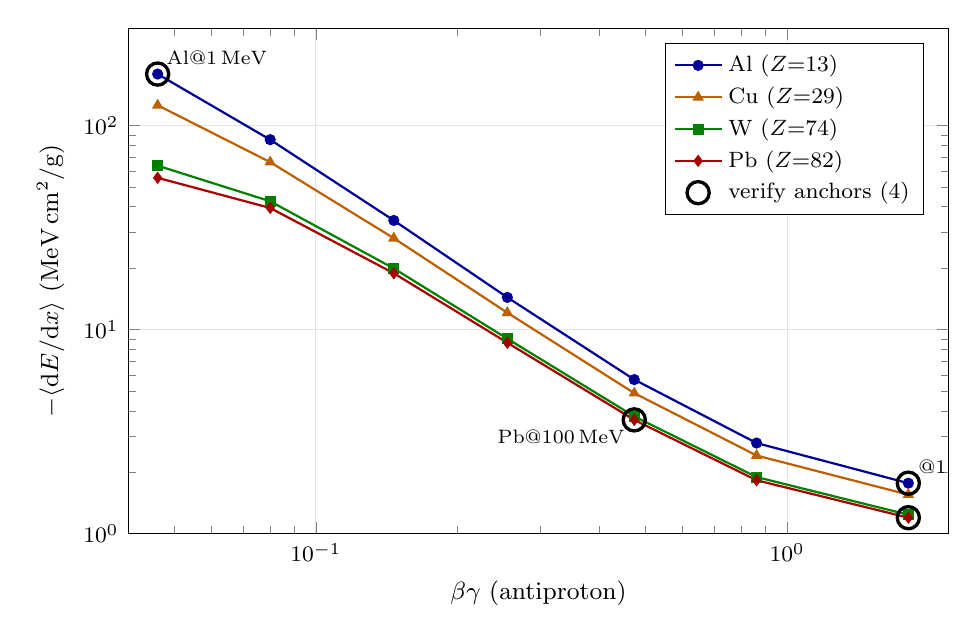
\begin{tikzpicture}
\begin{axis}[
  width=12cm, height=8cm,
  xmode=log, ymode=log,
  xlabel={$\beta\gamma$ (antiproton)},
  ylabel={$-\langle\mathrm{d}E/\mathrm{d}x\rangle$ (MeV\,cm$^2$/g)},
  xmin=0.04, xmax=2.2,
  ymin=1.0, ymax=300,
  legend pos=north east,
  legend cell align=left,
  legend style={font=\footnotesize},
  tick label style={font=\footnotesize},
  label style={font=\small},
  ymajorgrids, xmajorgrids,
  grid style={gray!22},
  mark size=1.6pt,
]
% Al
\addplot[blue!60!black, thick, mark=*] coordinates {
  (0.04618131,178.82465) (0.08003097,85.26499) (0.14638774,34.27874)
  (0.25489145,14.38117) (0.47383209,5.68688) (0.86122291,2.77939)
  (1.80761829,1.76663)
};
\addlegendentry{Al ($Z{=}13$)}
% Cu
\addplot[orange!75!black, thick, mark=triangle*] coordinates {
  (0.04618131,125.75020) (0.08003097,66.17186) (0.14638774,28.04244)
  (0.25489145,12.09958) (0.47383209,4.88009) (0.86122291,2.41455)
  (1.80761829,1.55205)
};
\addlegendentry{Cu ($Z{=}29$)}
% W
\addplot[green!50!black, thick, mark=square*] coordinates {
  (0.04618131,63.61595) (0.08003097,42.54863) (0.14638774,19.93620)
  (0.25489145,9.02214) (0.47383209,3.75537) (0.86122291,1.89332)
  (1.80761829,1.23748)
};
\addlegendentry{W ($Z{=}74$)}
% Pb
\addplot[red!65!black, thick, mark=diamond*] coordinates {
  (0.04618131,55.46333) (0.08003097,39.46452) (0.14638774,18.88240)
  (0.25489145,8.62331) (0.47383209,3.60999) (0.86122291,1.82608)
  (1.80761829,1.19698)
};
\addlegendentry{Pb ($Z{=}82$)}
% the 4 verify-ledger reference anchors (black ringed)
\addplot[only marks, mark=o, mark size=4pt, draw=black, very thick] coordinates {
  (0.04618131,178.82465)   % Al @ 1 MeV
  (1.80761829,1.76663)     % Al @ 1 GeV
  (0.47383209,3.60999)     % Pb @ 100 MeV
  (1.80761829,1.19698)     % Pb @ 1 GeV
};
\addlegendentry{verify anchors (4)}
\node[font=\scriptsize,anchor=south west] at (axis cs:0.046,178.8) {Al@1\,MeV};
\node[font=\scriptsize,anchor=north east] at (axis cs:0.474,3.61) {Pb@100\,MeV};
\node[font=\scriptsize,anchor=south west] at (axis cs:1.81,1.77) {@1\,GeV};
\end{axis}
\end{tikzpicture}
\end{document}
